\documentclass[compress]{beamer}
\usepackage{ifthen,verbatim}

\newcommand{\isnote}{}
\xdefinecolor{lightyellow}{rgb}{1.,1.,0.25}
\xdefinecolor{darkblue}{rgb}{0.1,0.1,0.7}

%% Uncomment this to get annotations
%% \def\notes{\addtocounter{page}{-1}
%%            \renewcommand{\isnote}{*}
%% 	   \beamertemplateshadingbackground{lightyellow}{white}
%%            \begin{frame}
%%            \frametitle{Notes for the previous page (page \insertpagenumber)}
%%            \itemize}
%% \def\endnotes{\enditemize
%% 	      \end{frame}
%%               \beamertemplateshadingbackground{white}{white}
%%               \renewcommand{\isnote}{}}

%% Uncomment this to not get annotations
\def\notes{\comment}
\def\endnotes{\endcomment}

\setbeamertemplate{navigation symbols}{}
\setbeamertemplate{headline}{\mbox{ } \hfill
\begin{minipage}{5.5 cm}
\vspace{-0.75 cm} \small
\end{minipage} \hfill
\begin{minipage}{4.5 cm}
\vspace{-0.75 cm} \small
\begin{flushright}
\ifthenelse{\equal{\insertpagenumber}{1}}{}{Jim Pivarski \hspace{0.2 cm} \insertpagenumber\isnote/\pageref{numpages}}
\end{flushright}
\end{minipage}\mbox{\hspace{0.2 cm}}\includegraphics[height=1 cm]{../cmslogo} \hspace{0.1 cm} \includegraphics[height=1 cm]{../tamulogo} \hspace{0.01 cm} \vspace{-1.05 cm}}

\begin{document}
\begin{frame}
\vfill
\begin{center}
\textcolor{darkblue}{\Large Muon and Tracker Alignment at Start-Up}

\vfill
\begin{columns}
\column{0.3\linewidth}
\begin{center}
\large
\textcolor{darkblue}{Jim Pivarski}
\end{center}
\end{columns}

\begin{columns}
\column{0.3\linewidth}
\begin{center}
\scriptsize
{\it Texas A\&M University}
\end{center}
\end{columns}

\vfill
 8 December, 2009

\end{center}
\end{frame}

%% \begin{notes}
%% \item This is the annotated version of my talk.
%% \item If you want the version that I am presenting, download the one
%% labeled ``slides'' on Indico (or just ignore these yellow pages).
%% \item The annotated version is provided for extra detail and a written
%% record of comments that I intend to make orally.
%% \item Yellow notes refer to the content on the {\it previous} page.
%% \item All other slides are identical for the two versions.
%% \end{notes}

\small

\begin{frame}
\frametitle{Status of alignments}
\begin{itemize}\setlength{\itemsep}{0.1 cm}
\item Tracker alignment
\begin{itemize}\setlength{\itemsep}{0.1 cm}
\item CRAFT-09: repeated CRAFT-08 exercise, introduced prompt workflow (frequent, automated, low-statistics alignment)
\item Cooling incident: physically moved pixel half-shell 30~$\mu$m in $z$
\item Re-aligned using November cosmic rays, \textcolor{darkblue}{this is startup}
\end{itemize}

\item DT alignment
\begin{itemize}\setlength{\itemsep}{0.1 cm}
\item CRAFT-09: repeated CRAFT-08 exercise with tighter bounds on alignment uncertainties, \textcolor{darkblue}{this is startup}
\item Barrel hardware alignment is now producing alignments; testing with tracks
\end{itemize}

\item CSC alignment
\begin{itemize}\setlength{\itemsep}{0.1 cm}
\item CRAFT-09: corrected few-mm disk position errors with tracks,
  hardware system providing missing degrees of freedom, \\
  \textcolor{darkblue}{this is startup}
\item New LHC runs provide too few beam-halo tracks \mbox{for alignment\hspace{-1 cm}}
\end{itemize}
\end{itemize}
%% \hspace{-0.83 cm} \textcolor{darkblue}{\Large Outline2}
\end{frame}

\begin{frame}
\frametitle{Tracker cooling incident}

\begin{itemize}
\item Below: module position differences before and after cooling incident

\item Left: ``after'' = prompt alignment performed immediately after
  incident (low statistics, but pinpoints the motion in time)

\item Right: ``after'' = full-statistics November cosmic ray alignment
\end{itemize}

\includegraphics[width=\linewidth]{pxb_motion.png}
\end{frame}

\begin{frame}
\frametitle{Tracker alignment statistics}

\begin{itemize}\setlength{\itemsep}{0.25 cm}
\item Month-long CRAFT: $\sim$3 million tracks after quality cuts

\item November cosmics \textcolor{darkblue}{(startup)}: $\sim$2 million
\begin{itemize}
\item roughly the same quality in strip tracker
\item pixel (smaller target for cosmic rays): 2--2.5~$\mu$m (nearly
  ideal) in CRAFT but 3--4~$\mu$m in startup alignment

{\scriptsize (RMS of distribution of median of residuals, measure of local precision)}
\end{itemize}

\item About 10~M quality minbias tracks needed to improve alignment
\end{itemize}

\vfill
\hspace{-0.83 cm} \textcolor{darkblue}{\Large Tracker alignment systematics}

\vspace{0.1 cm}
\begin{itemize}
\item Combining data with different topologies (minbias, cosmics) and
  introducing new constraints (primary vertex, resonances) yields
  qualitatively new information on the global shape of the tracker
\end{itemize}
\end{frame}

\begin{frame}
\frametitle{Other outstanding tracker issues}

\begin{itemize}
\item 5~mm gap between two half-cylinders of TIB (known since first alignments at the Tracker Integration Facility)

\item Want to see if tracks from collisions confirm the observation
\end{itemize}

\includegraphics[width=\linewidth]{tib_gap.png}

\begin{itemize}
\item Minbias illuminate the tracker endcaps better than cosmics
\begin{itemize}
\item the last TEC disk is used to connect tracker to muon hardware alignment system
\item improved tracker endcap $\to$ improved hardware alignment global position
\end{itemize}
\end{itemize}

\textcolor{blue}{\scriptsize https://twiki.cern.ch/twiki/bin/view/CMS/TrackerAlignmentWithBeams2009}
\end{frame}

\begin{frame}
\frametitle{Studying tracker with muon hits}

\vspace{0.25 cm}
\begin{columns}
\column{0.4\linewidth}
\includegraphics[width=\linewidth]{method.pdf}

\column{0.7\linewidth}
\begin{itemize}
\item As an external detector, the muon system can analyze global distortions in the tracker
\item Select one DT layer to simplify and minimize dependence on muon alignment
\item Varying DT layer position maps a family of curves for tracker momentum error \mbox{($\Delta p_T/p_T$)\hspace{-1 cm}}
\end{itemize}
\end{columns}

\vspace{0.25 cm}
\includegraphics[width=0.5\linewidth]{residuals_real_both.pdf}\mbox{\hspace{0.2 cm}}\includegraphics[width=0.5\linewidth]{momenta_real_both.pdf}

\vspace{-0.25 cm}
\begin{itemize}
\item More details in the Alignment \& Calibration meeting today
\end{itemize}
\end{frame}

\begin{frame}
\frametitle{DT startup from CRAFT-09}

\begin{columns}
\column{0.6\linewidth}
\mbox{Repeated all checks developed for CRAFT-08\hspace{-1 cm}}

\begin{itemize}
\item Right: lots of plots

\item Below: local segment cross-check
\begin{itemize}
\item now includes full propagation between stations (not linear)
\item 0.70~mm upper bound on local alignment error $\to$ 0.35~mm for
  stations 1--3
\end{itemize}
\end{itemize}

\vfill
\includegraphics[height=\linewidth, angle=90]{NOV4_segdiff_x_whze.pdf}

\column{0.4\linewidth}
\vspace{-1 cm}
\hfill \includegraphics[width=0.8\linewidth]{MBwhCst1sec10_bellcurves.png}

\includegraphics[width=\linewidth]{MBwhCst1sec10_polynomials.png}

\includegraphics[width=\linewidth]{DTvsphi_st1whC_x.png}

\includegraphics[height=\linewidth, angle=90]{NOV4DT_median_goodDT.pdf}
\end{columns}
\end{frame}

\begin{frame}
\frametitle{Cosmic splitting results}

\mbox{\hspace{-0.85 cm}
\includegraphics[width=0.6\linewidth]{StandAlone.png}
\includegraphics[width=0.6\linewidth]{GlobalMuon.png}}

\mbox{ } \hfill {\scriptsize \textcolor{darkblue}{J.~Tucker}}

\vfill
\begin{itemize}
\item DT alignment yields clear improvement in standAloneMuons (left)
  and globalMuons (right), with little difference between globalMuon
  and FirstMuonStation (4.2\% vs.\ 4.0\% at 200~GeV)
\item standAloneMuon resolution is still valid
\item muon alignment may need to be repeated to regain globalMuon resolution
\end{itemize}
\end{frame}

\begin{frame}
\frametitle{Barrel hardware alignment}

\begin{columns}
\column{0.7\linewidth}
\includegraphics[height=\linewidth, angle=90]{NOV4DT_vs_HARDWARE_phi.pdf}

\includegraphics[width=\linewidth]{NovHardware_vs_phi.pdf}

\column{0.4\linewidth}
\begin{itemize}
\item Differences in chamber positions between hardware and track-based geometries
\only<1>{\item Top-left: reconstruction was following some LED reflections}
\only<1>{\item Bottom-left: corrected}
\only<2>{\item Sine curve: global position with respect to tracker
\begin{itemize}
\item $x \to 1.2$~mm
\item $y \to 4.5$~mm
\item $\phi_z \to 0.58$~mrad
\end{itemize}}
\end{itemize}

\only<1>{\includegraphics[width=\linewidth]{hwbarrel_spots.png}}
\only<2>{\includegraphics[width=\linewidth]{adjustment_cartoon.pdf}}
\end{columns}
\end{frame}

\begin{frame}
\frametitle{CSC startup from CRAFT-09}

\begin{itemize}
\item Largest correction: positions of disks after closing
\item Important step after beam-halo alignment, to locate internally-aligned rings with respect to tracker
\end{itemize}

\begin{columns}
\column{0.4\linewidth}
\includegraphics[width=\linewidth]{tracker_disk_interpretation.pdf}

\column{0.6\linewidth}
\includegraphics[height=0.95\linewidth, angle=90]{ringfits_before_mem12.pdf}

\includegraphics[height=0.95\linewidth, angle=90]{ringfits_after_mem12.pdf}
\end{columns}
\end{frame}

\begin{frame}
\frametitle{Endcap hardware alignment}

\begin{columns}

\column{0.6\linewidth}
\begin{itemize}
\item Hardware geometry provides $z$ and $\phi_x$ (tracks are insensitive to these)
\item Reconstruction recently extended to transfer lines (inter-disk)
  and $r\phi$ positions of monitored chambers
\item Opportunity to compare $r\phi$ with tracks
\end{itemize}

\includegraphics[width=\linewidth]{slm_lines.png}

\column{0.4\linewidth}
\vspace{1 cm}
\mbox{ }

Laser line residuals: internal consistency of hardware alignment

\includegraphics[width=\linewidth]{hw_rphi_residuals.png}
\end{columns}
\end{frame}

\begin{frame}
\frametitle{Beam-halo!  But not many\ldots}
\begin{columns}
\column{0.7\linewidth}
\includegraphics[width=0.9\linewidth]{trigger_plot.png}

\column{0.4\linewidth}
\begin{itemize}\setlength{\itemsep}{-0.05 cm}
\item Longest period of true beam-halo: 13~min in run 122294
\item Overlaps track yield: 229 in outer ring after sensible cuts
\item Not enough for alignment
\end{itemize}
\end{columns}

\vspace{-0.3 cm}
\includegraphics[height=4 cm]{occupancy_121964_122294.pdf}
\includegraphics[height=4.5 cm]{overlaps_xypos_121964_122294.pdf}
\end{frame}

\begin{frame}
\frametitle{New beam-halo residuals}
\begin{columns}
\column{0.35\linewidth}
\includegraphics[width=\linewidth]{residuals_diagrams.pdf}

\column{0.65\linewidth}
\begin{itemize}
\item Two types of residuals: continuity ($\Delta r\phi$) and differentiability ($\Delta \frac{d(r\phi)}{dz}$)
\item Outer ring consistent with $\sim$1~mm RMS misalignment
\end{itemize}
\end{columns}

\begin{center}
\includegraphics[width=0.8\linewidth]{outer_residuals.pdf}
\end{center}
\end{frame}

\begin{frame}
\frametitle{Upcoming alignment steps}

\textcolor{darkblue}{\large Very soon (this year?)}

\begin{itemize}
\item Tracker: combine cosmics and minbias with primary vertex constraint, beam-halo
\item DT: continue aligning with cosmic rays
\item CSC: align chambers relative to ring with beam-halo, rings relative to tracker with cosmics
\end{itemize}

\textcolor{darkblue}{\large Larger datasets ($\sim$5~pb$^{-1}$)}

\begin{itemize}
\item Tracker: add isolated muon, $J/\psi$, $\Upsilon$
\item DT: combine cosmics and collisions muons
\item CSC: use collisions for chambers-in-ring and tracker-to-ring (cross-checks)
\end{itemize}

\textcolor{darkblue}{\large Even larger}

\begin{itemize}
\item DT and CSC together, using standard algorithm
\end{itemize}
\end{frame}

\begin{frame}
\frametitle{MC studies of alignment reach}
\begin{itemize}
\item \textcolor{darkblue}{Aysen Tatarinov (TAMU)}, new muon alignment expert in training

\item Studied alignment resolution as a function of integrated luminosity using standard algorithm
\begin{itemize}
\item aligning all chambers with more than 30 tracks
\item RMS $r\phi$ resolution {\it for the aligned chambers}
\item see backup for full results
\end{itemize}
\end{itemize}

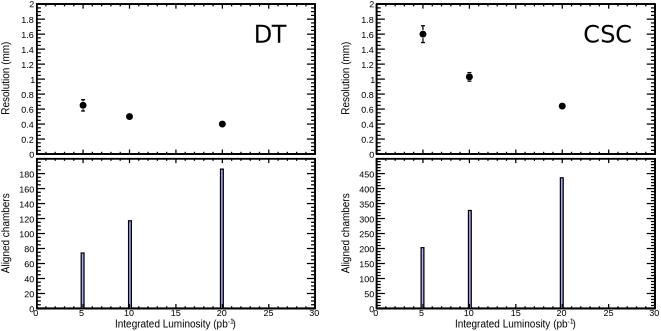
\includegraphics[width=\linewidth]{aysens_results.pdf}
\end{frame}

\begin{frame}
\frametitle{Distribution of aligned chambers}

\begin{itemize}
\item The alignment fitter succeeds for more chambers as integrated luminosity is added

\item Complements chambers accessible with cosmic rays
\end{itemize}

\vspace{-0.6 cm}
\begin{columns}
\column{0.32\linewidth}

\begin{center}
5~pb$^{-1}$
\end{center}

\vspace{-0.45 cm}
\includegraphics[width=\linewidth]{il05_DT_fraction.png}

\includegraphics[width=\linewidth]{il05_CSC_fraction.png}

\column{0.32\linewidth}

\begin{center}
10~pb$^{-1}$
\end{center}

\vspace{-0.4 cm}
\includegraphics[width=\linewidth]{il10_DT_fraction.png}

\includegraphics[width=\linewidth]{il10_CSC_fraction.png}

\column{0.32\linewidth}

\begin{center}
20~pb$^{-1}$
\end{center}

\vspace{-0.4 cm}
\includegraphics[width=\linewidth]{il20_DT_fraction.png}

\includegraphics[width=\linewidth]{il20_CSC_fraction.png}

\end{columns}

\end{frame}

%% \section*{First section}
%% \begin{frame}
%% \begin{center}
%% \Huge \textcolor{blue}{First section}
%% \end{center}
%% \end{frame}

\begin{frame}
\frametitle{Conclusions}
\begin{itemize}\setlength{\itemsep}{0.5 cm}
\item Tracker CRAFT alignment is precise, but cooling incident moved things; current alignment is post-incident
\begin{itemize}
\item \scriptsize new project: analyzing tracker global distortions with the muon system; \\ if you're interested, more details in Alignment \& Calibration meeting
\end{itemize}

\item Current DT + CSC alignments based on CRAFT-09

\item Hardware geometry is being studied with tracks (right now for
  barrel and soon for endcap)

\item Too few beam-halo muons for alignment, but the tracks we do see
  have the right distributions

\item Aysen: new aligner in the group, quantifying resolution with low-lumi samples

\end{itemize}
\label{numpages}
\end{frame}

\begin{frame}
\frametitle{DT 5~~pb$^{-1}$}
\includegraphics[width=0.8\linewidth]{il05_DT_00.png}
\end{frame}

\begin{frame}
\frametitle{CSC 5~~pb$^{-1}$}
\includegraphics[width=0.8\linewidth]{il05_CSC_00.png}
\end{frame}

\begin{frame}
\frametitle{DT 10~pb$^{-1}$}
\includegraphics[width=0.8\linewidth]{il10_DT_00.png}
\end{frame}

\begin{frame}
\frametitle{CSC 10~pb$^{-1}$}
\includegraphics[width=0.8\linewidth]{il10_CSC_00.png}
\end{frame}

\begin{frame}
\frametitle{DT 20~pb$^{-1}$}
\includegraphics[width=0.8\linewidth]{il20_DT_00.png}
\end{frame}

\begin{frame}
\frametitle{CSC 20~pb$^{-1}$}
\includegraphics[width=0.8\linewidth]{il20_CSC_00.png}
\end{frame}

\end{document}
